\documentclass[a4paper,11pt]{article}
\usepackage[T1]{fontenc}
\usepackage[utf8]{inputenc}
\usepackage{lmodern}
\usepackage{graphicx}
\usepackage{amsmath}
\usepackage{amsfonts}
\usepackage{amssymb}
\usepackage{mathtools}
\usepackage{epstopdf}

\DeclareMathOperator{\given}{\mid}

\begin{document}

\section*{HW1}

\begin{tabular*}{0.9\textwidth}{@{\extracolsep{\fill} } lll}
Jimmy Hold\"{o} & & Jared Karr\\
890130-6319 & & 801120-4693\\
\it{gusholji@student.gu.se} & & \it{karr@student.chalmers.se}\\
\end{tabular*}

\section{Theoretical problems}
\subsection{Maximum likelihood estimator (MLE)}
The likelihood of a set of observations $\mathbf{x_1},\dots,\mathbf{x_n}\in\mathbb{R}^p$ drawn I.I.D. from a $p$-dimensional spherical Gaussian distribution having mean $\boldsymbol\mu\in\mathbb{R}^p$ and variance $\sigma^2\in\mathbb{R}_{>0}$ is
\begin{align*}
  P(\mathbf{x_1},\dots,\mathbf{x_n}\given \boldsymbol\mu,\sigma^2)
    &=\prod_{i=1}^n\mathcal{N}(\mathbf{x_i}\given \boldsymbol\mu, \sigma^2)\\
    &=\prod_{i=1}^n\left(
        \frac{1}{\sqrt{2\pi}\sigma}
      \right)^p\exp\left(
        \frac{-(\mathbf{x_i}-\boldsymbol\mu)^\top(\mathbf{x_i}-\boldsymbol\mu)}
             {2\sigma^2}
      \right).
\end{align*}
To find $\sigma_\mathrm{MLE}$, it is easier to maximize the log-likelihood
\begin{equation*}
  \log P(\mathbf{x_1},\dots,\mathbf{x_n}\given\boldsymbol\mu,\sigma^2)
    =\sum_{i=1}^n
      -p\log\sqrt{2\pi}
      -p\log\sigma
      -\frac{(\mathbf{x_i}-\boldsymbol\mu)^\top(\mathbf{x_i}-\boldsymbol\mu)}{2\sigma^2} 
\end{equation*}
with respect to $\sigma$. Taking the appropriate partial derivative and setting to zero,
\begin{align*}
\frac{\partial\log P}{\partial\sigma}
  &=\sum_{i=1}^n
    -\frac{p}{\sigma}
    +\frac{1}{\sigma^3}\cdot(\mathbf{x_i}-\boldsymbol\mu)^\top(\mathbf{x_i}-\boldsymbol\mu)\\
  &=-\frac{np}{\sigma}
    +\frac{1}{\sigma^3}\sum_{i=1}^n(\mathbf{x_i}-\boldsymbol\mu)^\top(\mathbf{x_i}-\boldsymbol\mu)=0\\
np\sigma^2
  &=\sum_{i=1}^n(\mathbf{x_i}-\boldsymbol\mu)^\top(\mathbf{x_i}-\boldsymbol\mu)\\
\sigma_\mathrm{MLE}&=\sqrt{\frac{1}{np}\sum_{i=1}^n(\mathbf{x_i}-\boldsymbol\mu_\mathrm{MLE})^\top(\mathbf{x_i}-\boldsymbol\mu_\mathrm{MLE})}.
\end{align*}

\subsection{Posterior distributions}

\paragraph{(a)} Bayes rule gives the posterior distribution
\begin{align*}
  P(s\given \mathbf{x_1},\dots,\mathbf{x_n};\alpha,\beta)
    &=\frac{
        P(\mathbf{x_1},\dots,\mathbf{x_n}\given s)P(s\given\alpha,\beta)
      }{
        \int_{s=0}^\infty P(\mathbf{x_1},\dots,\mathbf{x_n}\given s)P(s\given\alpha,\beta)\,ds
      },
\end{align*}
but we can ignore the normalization constants of each distribution to simplify the expression:
\begin{align*}
  P(s\given \mathbf{x_1},\dots,\mathbf{x_n};\alpha,\beta)
    &\propto P(\mathbf{x_1},\dots,\mathbf{x_n}\given s)P(s\given\alpha,\beta)\\
    &\propto
      \prod_{i=1}^n \left(
        s^{-1}\exp\left(-\frac{(\mathbf{x_i}-\boldsymbol\mu)^\top(\mathbf{x_i}-\boldsymbol\mu)}{2s}\right)
      \right)
      \cdot
      s^{-\alpha-1}\exp\left(-\frac{\beta}{s}\right)\\
    &\propto
      s^{-n-\alpha-1}
      \exp\left(
        \frac{
          -\beta
          -\frac{1}{2}\left(
            \sum_{i=1}^n
              (\mathbf{x_i}-\boldsymbol\mu)^\top(\mathbf{x_i}-\boldsymbol\mu)
          \right)
        }{
          s
        }
      \right)\\
    &\propto
      s^{-{\alpha+n}-1}
      \exp\left(
        \frac{
          -(\beta+n\sigma_\mathrm{MLE}^2)
        }{
          s
        }
      \right).
\end{align*}
Let $\alpha'=\alpha+n$ and $\beta'=\beta+n\sigma_\mathrm{MLE}^2$, then the posterior distribution takes the same form as the prior:
\begin{align*}
P(s\given \mathbf{x_1},\dots,\mathbf{x_n};\alpha,\beta)
  &=P(s\given\alpha',\beta')\\
  &=\frac{{\beta'}^{\alpha'}}{\Gamma(\alpha')}s^{-\alpha'-1}\exp\left(\frac{-\beta'}{s}\right)
\end{align*}

\paragraph{(b)} The Bayes factor between models $M_A$ and $M_B$ is defined to be
\begin{align*}
\mathrm{BF}&=
  \frac{
    P(\mathbf{x_1},\dots,\mathbf{x_n}\given\alpha_A,\beta_A)
  }{
    P(\mathbf{x_1},\dots,\mathbf{x_n}\given\alpha_B,\beta_B)
  }.
\end{align*}
From Bayes rule, we get
\begin{align*}
\mathrm{BF}&=
  \frac{
    \frac{
      P(\mathbf{x_1},\dots,\mathbf{x_n}\given s)P(s\given\alpha_A,\beta_A)      
    }{
      P(s\given\alpha_A',\beta_A')
    }
  }{
    \frac{
      P(\mathbf{x_1},\dots,\mathbf{x_n}\given s)P(s\given\alpha_B,\beta_B)      
    }{
      P(s\given\alpha_B',\beta_B')
    }
  }\\
&=
  \frac{
    P(s\given\alpha_A,\beta_A)P(s\given\alpha_B',\beta_B')
  }{
    P(s\given\alpha_A',\beta_A')P(s\given\alpha_B,\beta_B)
  }\\
&=
  \frac{
    \beta_A^{\alpha_A}\beta_B'^{\alpha_B'}
    \Gamma(\alpha_A')\Gamma(\alpha_B)
  }{
    \beta_A'^{\alpha_A'}\beta_B^{\alpha_B}
    \Gamma(\alpha_A)\Gamma(\alpha_B')
  }
  \cdot
  s^{\alpha_A'-\alpha_A+\alpha_B-\alpha_B'}
  \exp\left(
    \frac{
      \beta_A'-\beta_A+\beta_B-\beta_B'
    }{
      s
    }
  \right)
\end{align*}
Note that the posterior models $(\alpha_A', \beta_A')$ and $(\alpha_B', \beta_B')$ incorporate the same evidence, so that
\begin{align*}
  \alpha_A'-\alpha_A+\alpha_B-\alpha_B'&=
  \alpha_A+n-\alpha_A+\alpha_B-\alpha_B-n=0\\
  \intertext{and}
  \beta_A'-\beta_A+\beta_B-\beta_B'&=
  \beta_A+n\sigma_\mathrm{MLE}^2-\beta_A+\beta_B-\beta_B-n\sigma_\mathrm{MLE}^2=0,
\end{align*}
causing the terms involving $s$ to disappear from the Bayes factor:
\begin{align*}
\mathrm{BF}&=
  \frac{
    \beta_A^{\alpha_A}\beta_B'^{\alpha_B'}
    \Gamma(\alpha_A')\Gamma(\alpha_B)
  }{
    \beta_A'^{\alpha_A'}\beta_B^{\alpha_B}
    \Gamma(\alpha_A)\Gamma(\alpha_B')
  }
\end{align*}
\paragraph{(c)}

\section{Practical problems}
\subsection{Spherical Gaussian estimation}
\paragraph{(a)}
\begin{align*}
\boldsymbol\mu_\mathrm{MLE}&=\frac{1}{n}\sum_{i=1}^n\mathbf{x_i}\\
\sigma_\mathrm{MLE}&=\sqrt{\frac{1}{np}\sum_{i=1}^n(\mathbf{x_i}-\boldsymbol\mu_\mathrm{MLE})^\top(\mathbf{x_i}-\boldsymbol\mu_\mathrm{MLE})}.
\end{align*}
\paragraph{(d)}
\begin{figure}
  \begin{center}
    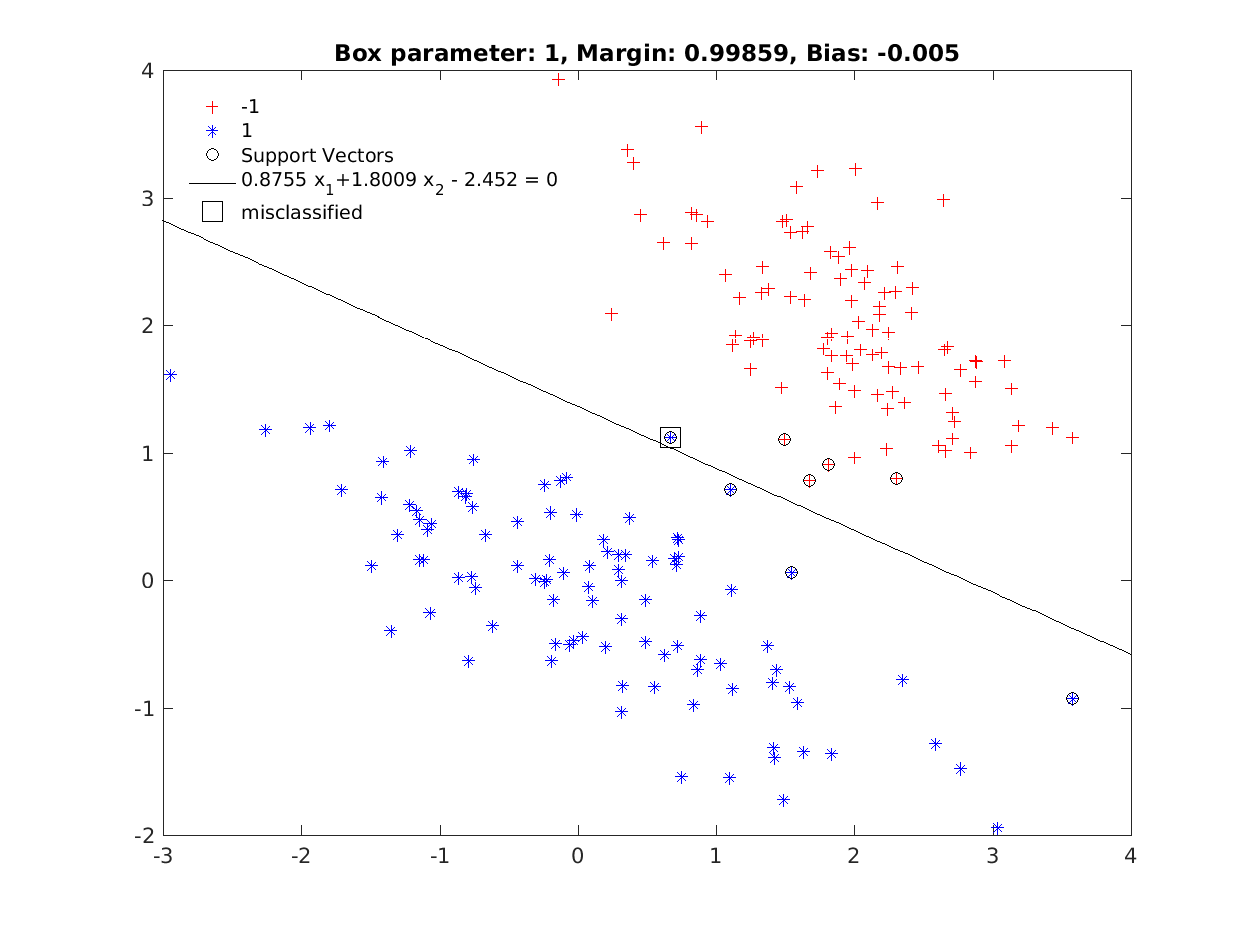
\includegraphics[width=\textwidth]{P2_1}
  \end{center}
\end{figure}
\subsection{MAP estimation}
\end{document}
